\documentclass{article}

\usepackage[margin=0.75in]{geometry}
\usepackage{amsmath,amsthm,amssymb}
\usepackage{graphicx,float}
\usepackage{multirow,setspace}
\usepackage{natbib,enumerate}
\usepackage{caption}
\usepackage{subcaption}
\usepackage{termcal} 
\usepackage{xcolor}
\usepackage{enumitem}
\usepackage{gensymb}
\usepackage{multicol}
\usepackage{listings}
\usepackage{booktabs}
\usepackage{hyperref}
\usepackage{listings}
\usepackage{xcolor}


\setlength{\marginparwidth}{2cm}

\renewcommand{\thesection}{\Alph{section}}
\newcommand{\HRule}{\rule{\linewidth}{0.5mm}}
\newcommand{\tab}{\hspace{0.5cm}}
\newcommand{\modref}[1]{(\ref{#1})}

\newcommand{\bbeta}{{\mbox{\boldmath$\beta$}}}
\newcommand{\bmu}{{\mbox{\boldmath$\mu$}}}
\newcommand{\balpha}{{\mbox{\boldmath$\alpha$}}}
\newcommand{\btheta}{{\mbox{\boldmath$\theta$}}}
\newcommand{\bpi}{{\mbox{\boldmath$\pi$}}}
\newcommand{\R}{\texttt{R}}
\newcommand{\Lik}{\mathcal{L}}

\captionsetup[subfigure]{labelformat=empty}

\begin{document}

%%% HEADER %%%
	\begin{center}
		\HRule \\[0.1cm]
		\vspace{0.1cm}
		{ \LARGE \bfseries MATH 2625: Biostatistical Methods\\[0.5cm] Homework 5, due Thursday, April 10 } \\[0.1cm]
		\HRule \\[0.1cm]
	\end{center}
	
		Please submit a PDF or .doc version of your homework to Canvas by 3:30pm on the due date. Please type \emph{all} responses. You are encouraged to use \R\ for all calculations.
		
	\section*{Theory}
	\begin{enumerate}
		\item Find the estimated parametric survivor, hazard, and cumulative hazard functions for each of the following distributions. Because these distributions require root finding algorithms to find the MLE for some of their parameters, we will fix those parameters at the values specified below. Please show all of your work.
		\begin{enumerate}
			\item $T_i \sim Pa(\mu, \alpha)$ for $i = 1, \ldots, n$, $\mu = T_{(1)}$ (i.e. the minimum survival time), and $\alpha$ unknown.
			\item $T_i \sim W(\lambda, \gamma)$  for $i = 1, \ldots, n$, $\gamma = 2$, and $\lambda$ unknown.
		\end{enumerate}
	\end{enumerate}

	\begin{proof}
	The pdf of $T_i \sim Pa(\mu, \alpha)$ is defined as

	\[ f(t) = \frac{\alpha\mu^\alpha}{t^{\alpha + 1}}.\] % pareto distribution PDF

	We can integrate $f(t)$ to find the cdf, $F(t)$.

	\begin{align*}
		F(t) = \int_{\mu}^{t} f(t)dt & = \int_{\mu}^{t} \frac{\alpha\mu^\alpha}{t^{\alpha + 1}} dt \\
		& = 1 - \left( \frac{\mu}{t} \right)^\alpha .
	\end{align*} % pareto distribution CDF (line above)

	Then our survival function $S(t)$ is defined as

	\[S(t) = \left( \frac{\mu}{t} \right)^\alpha .\] % survival function here!!!

	The hazard function $h(t)$ of the Pareto distribution is then
	
	\[h(t) = \frac{ \frac{\alpha\mu^\alpha}{t^{\alpha + 1}} }{ \left( \frac{\mu}{t}\right) ^\alpha } .\]

	This simplifies to

	\[ h(t) = \frac{\alpha}{t}.\]

	Since the cumulative haazard function is the negative natural log of the survival function, this means

	\[ H(t) = -\alpha \log \left( \frac{\mu}{t} \right). \]

	
	Now we will use the method of maximum likelihood to estimate $\hat{\alpha}$. The likelihood function of the Pareto distribtuion is

	\[L(t) = \prod_{i = 1}^{i = n} \frac{\alpha\mu^\alpha}{t^{\alpha + 1}}\]

	The log-likelihood of this function is

	\[\ell(t) = n\log(\alpha) + \alpha n \ln(\mu) - \alpha\sum \log(t_i) - \sum \log(t_i).\]

	When we differentiate this, we get

	\[ \frac{n}{\alpha} + n \log\mu - \sum\log t_i.\]

	To find the maximum likelihood, we set this expression equal to zero, which results In

	\[\hat{\alpha} = \frac{n}{t(\sum\log t_i - n\log\mu ) }.\]

	Now to estimate, we set $\alpha = \hat{\alpha}$ for each of the equations.

	\[ \widehat{S(t)} = \left( \frac{\mu}{t} \right)^{\frac{n}{t(\sum\log t_i - n\log\mu ) } }. \]

	\[ \widehat{h(t)} = \frac{n}{t^2(\sum\log t_i - n\log\mu ) }. \]

	\[ \widehat{H(t)} = - \frac{n}{t(\sum\log t_i - n\log\mu ) } \log \left( \frac{\mu}{t} \right). \]
	\end{proof}


	\begin{proof}
		The pdf of $T_i \sim W(\lambda, \gamma)$ is defined as 

		\[ f(t) = \lambda\gamma t^{\gamma - 1} e^{-\lambda t^\gamma} \]

		When we set $\gamma = 2$, we get 

		\[ f(t) = 2\lambda t e^{-\lambda t^2} \]

		To find the cdf $F(t)$, we integrate this expression:

		\begin{align*}
			F(t) & = \int_{0}^{t} 2\lambda t e^{-\lambda t^2} dt \\
			& = 1 - e^{- \lambda t^2},
		\end{align*}

		where $t$ is greater than 0. This means the survivor function $S(t)$ is 

		\[ S(t) = e^{- \lambda t^2}. \]

		Then we can calculate the hazard function using the simplified formula $\frac{f(t)}{S(t)}$. This simplifies to

		\[ h(t) = 2\lambda t.\]
		
		Additionally, the cumulative hazard function (the negative natural log of the survival function) is 

		\[ H(t) = -\log(e^{-\lambda t^2} ) = \lambda t^2.\]

		Now we will find the maximum likelihood estimate. Starting from our previously defined probability density function, the likelihood function is defined as 

		\begin{align*}
			L(\lambda) & = \prod_{i = 1}^{n} 2\lambda t_i e^ {-\lambda t_i^2 } \\
			& = 2^n \lambda ^ n ( \prod t_i ) e^{\sum - \lambda t^2}.
		\end{align*}

		When we take the log-likelihood, we get

		\[ \ell (\lambda) = n\log (2) + n\log(\lambda) + \sum\log(t_i) + \sum-\lambda t_i^2 \]

		Then when we differentiate, we are left with 

		\[ -\frac{n}{\lambda} = \lambda^{n - 1}n \sum-t_i^2.\]

		Setting this equal to zero and solving, our maximum likelihood estimate of $\lambda$ with $\gamma = 2$ is defined as 

		\[ \hat{\lambda} = \sqrt[n]{ \frac{1}{\sum t_i^2} }. \]

		The estimates for the survival, hazard, and cumulative hazard functions are 

		\[ \widehat{S(t)} = e^{- t^2 \sqrt[n]{ \frac{1}{\sum t_i^2} } },\]

		\[ \widehat{h(t)} = 2t \sqrt[n]{ \frac{1}{\sum t_i^2} }, \]

		and
		\[ \widehat{H(t)} = t^2 \sqrt[n]{ \frac{1}{\sum t_i^2} }. \]
	
	\end{proof}

	\newpage
	\section*{Case Studies}
	For each of the following case studies, create a structured abstract no longer than 4 pages in length (including figures, tables, and references). The Background section is provided for each and should be included in your write-up. You must write the Methods, Results, and Conclusion sections. Code should be included in an appendix as well.

	\begin{enumerate}
		\item The first Case Study looks at bladder cancer, both its recurrence and death due to bladder cancer. The data can be found in the file \texttt{bladder.txt}. Variables include subject's \texttt{id}, \texttt{time} (to recurrence, death, or censored in months), first recurrence status (\texttt{status1}, coded 1 for first recurrence, 0 for censored or dead), death status (\texttt{status2}, coded 1 for dead, 0 for censored or first recurrence), \texttt{treatment} (code \texttt{placebo}, \texttt{pyridoxine}, and \texttt{thiotepa}), the \texttt{number} of initial \texttt{number} tumors (coded \texttt{One}, \texttt{Two or Three}, and \texttt{Four or More}), and the \texttt{size} of the largest tumor (coded \texttt{1cm}, \texttt{2cm to 3cm}, and \texttt{4cm or Larger}).
		
		\item The second Case Study examines the time to first and second recurrence of chronic granulomatous disease or CGD. As only a subset of the patients had the second recurrence, there are two datasets for this study: \texttt{cgd1.txt} (first recurrence data) and \texttt{cgd2.txt} (second recurrence data). The variables in both datasets have the same names. Variables include subejct's \texttt{id}, the \texttt{time} to recurrence of infection in days, \texttt{status} (1 for recurrence, 0 for censored), \texttt{treatment} (coded \texttt{rIFN-g} for gamma r-interferon, \texttt{placebo}), pattern of inheritance (\texttt{inherit}, coded \texttt{autosomal} or \texttt{X-linked}), and use of prophylactic antibiotics at study entry (\texttt{propylac}, coded 1 for yes, 0 for no).	
	\end{enumerate}

	\newpage
	\subsection*{Background} % move these around to fix indent

	Bladder cancer is a common type of cancer, typically beginning in the urothelial cells of the bladder. The cancer is often caught in the early stages and is easily treatable. However, even early-stage surgical interventions may not prevent recurrence. To evaluate the effectiveness of post-surgical treatments, we conducted a three arm study comparing the effects of treatment with pyridoxine, thiotepa, or placebo on the primary end point of recurrence. We also consider the secondary end point of death. The size of the initial tumor or the number of initial tumors may also impact both study endpoints. We enrolled 118 patients with confirmed bladder cancer whose tumors were surgically removed and followed them until recurrence, death, or both.


	\subsection*{Methods}
	118 patients with bladder cancer whose tumors were removed via surgery were selected for this randomized controlled trial. The subjects were randomly given one of three treatments: pyridoxine, thiotepa, or a placebo. We followed patients after their treatment to determine whether patients had a recurrence of bladder cancer. We also examined whether or not the patients died. While there was a possibility of patients developing both outcomes of interest, we only observed the outcome that came first. The subject was subsequently considered censored for the other outcome.

	We used Kaplan-Meier estimation to estimate the survival functions of recurrence of cancer as well as death for each of the three treatment groups. Estimates of the median time to tumor recurrence and death were also found when available. We used a Gehan-Breslow-Wilcoxon Test to determine whether there was a significant difference in the survival curves for both outcomes over time in subjects with each of the different treatments. We also used Kaplan-Meier estimation to conduct secondary analyses on the interaction on the time to cancer recurrence of two potential confounders: size of a subject’s initial tumor and the number of initial tumors in a subject. All analyses were done at the nominal level.

	\subsection*{Results}
	Among the 118 patients who were selected for the study, 32 received pyridoxine, 38 received thiotepa, and the remaining 48 formed the placebo control group. 17 of the subjects died under study observation, and 62 had a recurrence of bladder cancer. We observed the longest median time to cancer recurrence in patients receiving pyridoxine of 42 months. We did not observe a median survival time for patients receiving pyridoxine or the placebo, as the death counts in these two treatment arms were very low. However, with censored subjects taken into account, we estimated a median survival time for patients receiving thiotepa to be 59 months.

	% TABLE ONE
	\begin{table}[ht]
		\centering
		\footnotesize
		\caption*{\textbf{Table 1. Time to Cancer Recurrence \& Death of Patients by Treatment Group}}
		\begin{tabular}{@{}l l | l l | l l @{}}
			\toprule
			Treatment & \parbox[t]{2cm}{Number of\\ Patients} & \parbox[t]{2.5cm}{Observed\\ Recurrences} & \parbox[t]{3cm}{Median Time to\\ Recurrence (months)} & \parbox[t]{2.5cm}{Observed\\ Deaths} & \parbox[t]{3cm}{Median Time to\\ Death (months)} \\
			\midrule
			Pyridoxine & 32 & 15 & 42 & 6 & NA \\
			Thiotepa   & 38 & 18 & 26 & 6 & 59 \\
			Placebo    & 48 & 29 & 16 & 5 & NA \\
			\midrule
			Total      & 118 & 62 & & 17 & \\
			\bottomrule
		\end{tabular}
	\end{table}

	\begin{figure}[htbp]
		\centering
		\captionsetup{labelformat = empty}
		\begin{subfigure}[t]{0.32\textwidth}
			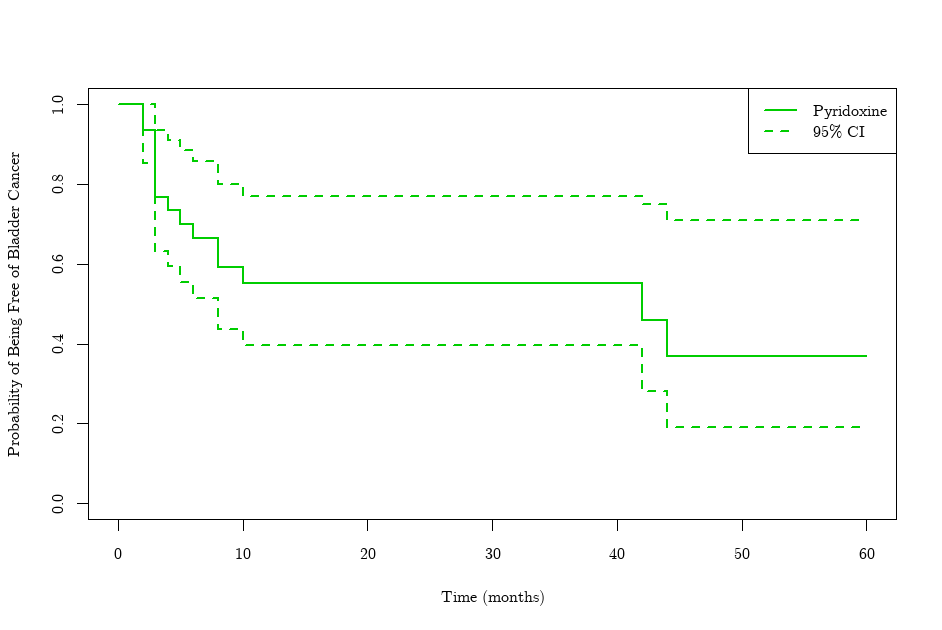
\includegraphics[width=\linewidth]{graphs/case1/recurrance~treatment_pyridoxine.png}
			\caption*{\raggedright\hyphenpenalty=10000\exhyphenpenalty=10000\sloppy 
			\textbf{Figure 1.} Time to Recurrence in Subjects Treated With Pyridoxine}
		\end{subfigure}
		\hfill
		\begin{subfigure}[t]{0.32\textwidth}
			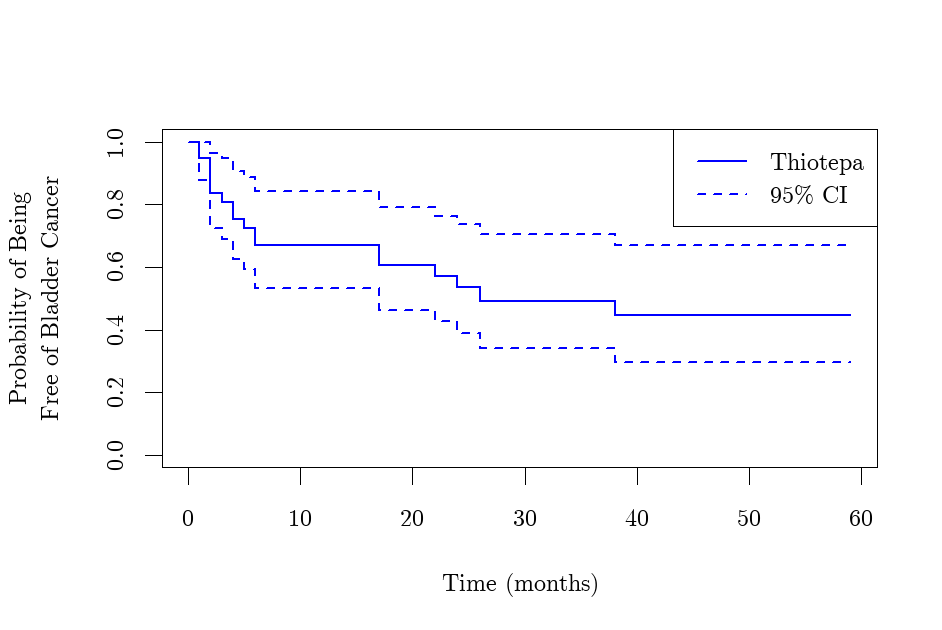
\includegraphics[width=\linewidth]{graphs/case1/recurrance~treatment_thiotepa.png}
			\caption*{\raggedright\hyphenpenalty=10000\exhyphenpenalty=10000\sloppy 
			\textbf{Figure 2.} Time to Recurrence in Subjects Treated With Thiotepa}
		\end{subfigure}
		\hfill
		\begin{subfigure}[t]{0.32\textwidth}
			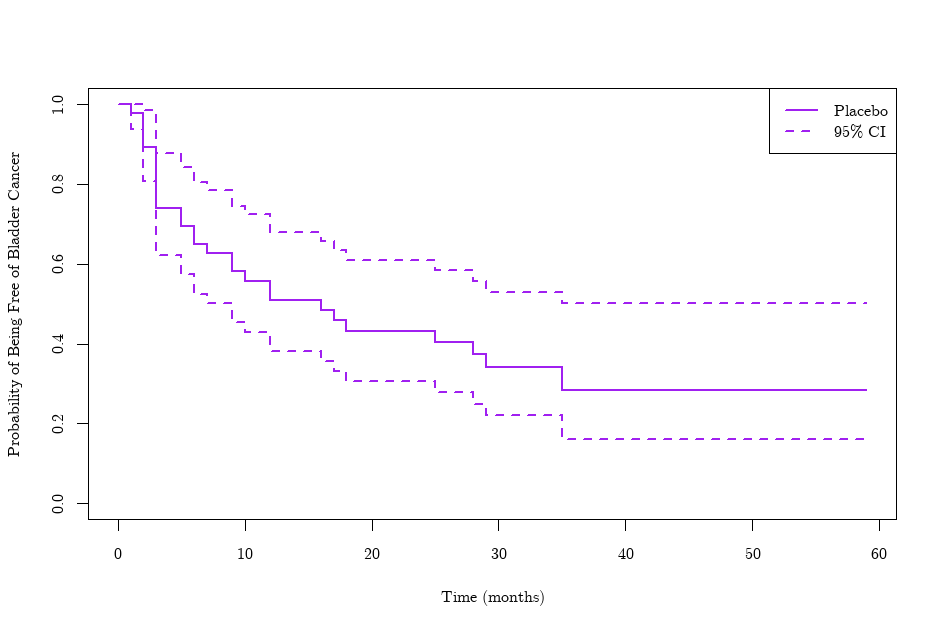
\includegraphics[width=\linewidth]{graphs/case1/recurrance~treatment_placebo.png}
			\caption*{\raggedright\hyphenpenalty=10000\exhyphenpenalty=10000\sloppy 
			\textbf{Figure 3.} Time to Recurrence in Control Group}
		\end{subfigure}
		\caption{Figures 1-3: Kaplan-Meier Estimates of Time to Bladder Cancer Recurrence for Each Treatment Group}
		\label{recur~treat_groups}
	  \end{figure} 
	  % Manually advance counter since we just "used" 3 figures
	  \addtocounter{figure}{2}
	  %%%%%%%%%%%%%%%%%%%%%%5

	% FIGURE FOUR: KAPLAN MEIER GRAPHS FOR ALL 3 TREATMENTS
	\begin{figure}[h!]
		\centering
		\tiny
		  \centering
		  \tiny
		  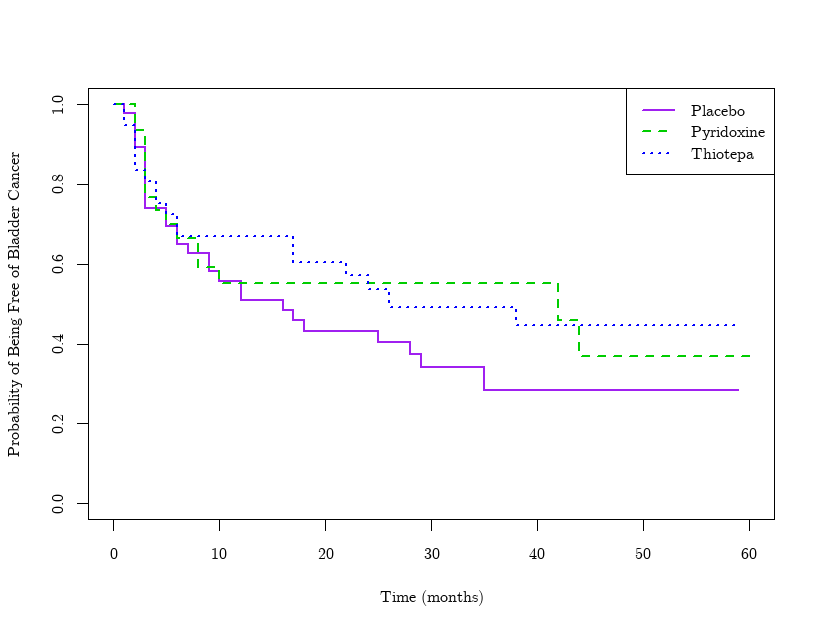
\includegraphics[width=0.6\textwidth]{graphs/case1/recurrance~treatment_all.png}
		  \caption{Kaplan-Meier Estimate of Time to Recurrence in Subjects by Treatment}
		  \label{recur~treat_all}
	\end{figure}

	  We did not find a statistically significant difference in recurrence rates over time between the three treatment groups $(p = 0.5, \chi^2 = 1.3$, df = 2). Figure 1 shows the Kaplan-Meier estimation of recurrence rates over time. We also did not find a significant difference in survival rates between the three treatment groups $(p = 0.8, \chi^2 = 0.5$, df = 2). Figure 5 shows Kaplan-Meier estimates of patient survival rates over time.

	  \begin{figure}[h!]
		\centering
		\tiny
		  \centering
		  \tiny
		  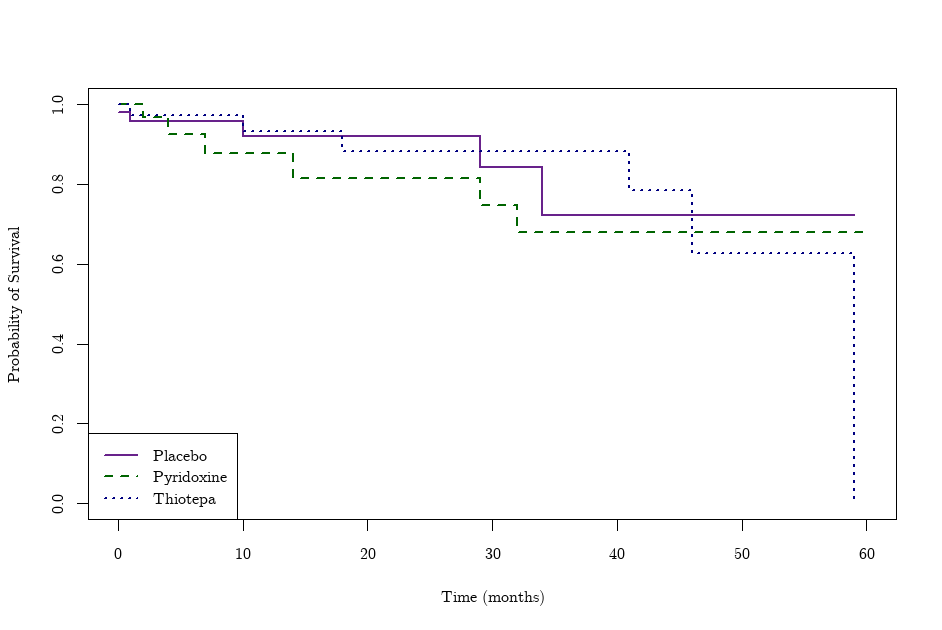
\includegraphics[width=0.6\textwidth]{graphs/case1/recurrance~death.png}
		  \caption{Kaplan-Meier Estimate of Survival Time in Subjects by Treatment}
		  \label{death~treat}
	\end{figure}

	\begin{table}[H]
		\centering
		\footnotesize
		\caption{\textbf{Time to Cancer Recurrence in Patients by Initial Number of Tumors}}
		\begin{tabular}{cccc}
			\toprule
			\multicolumn{1}{c}{Initial Number} & 
			\multicolumn{1}{c}{Number of} & 
			\multicolumn{1}{c}{Observed} & 
			\multicolumn{1}{c}{Median Time to} \\
			\multicolumn{1}{c}{of Tumors} & 
			\multicolumn{1}{c}{Patients} & 
			\multicolumn{1}{c}{Recurrences} & 
			\multicolumn{1}{c}{Recurrence (months)} \\
			\midrule
			One            & 72  & 30 & 42 \\
			Two to Three   & 27  & 17 & 24 \\
			Four or More   & 19  & 15 & 5  \\
			\midrule
			Total          & 118 & 62 &  \\
			\bottomrule
		\end{tabular}
	\end{table}

	\begin{table}[H]
		\centering
		\footnotesize
		\caption{\textbf{Time to Cancer Recurrence in Patients by Initial Size of Tumors}}
		\begin{tabular}{cccc}
			\toprule
			\multicolumn{1}{c}{Initial Size} & 
			\multicolumn{1}{c}{Number of} & 
			\multicolumn{1}{c}{Observed} & 
			\multicolumn{1}{c}{Median Time to} \\
			\multicolumn{1}{c}{of Tumors} & 
			\multicolumn{1}{c}{Patients} & 
			\multicolumn{1}{c}{Recurrences} & 
			\multicolumn{1}{c}{Recurrence (months)} \\
			\midrule
			1cm             & 69  & 38 & 22 \\
			2cm to 3cm      & 33  & 13 & N/A \\
			4cm or Larger   & 16  & 11 & 6  \\
			\midrule
			Total           & 118 & 62 &    \\
			\bottomrule
		\end{tabular}
	\end{table}

	While 72 of the 118 subjects only had one prior tumor present, 19 had at least four tumors. Additionally, most tumors were within 1cm in size, while only 16 patients had tumors larger than 4cm in size. Tables 2 and 3 provide a more detailed break-down of the findings. There was a statistically significant difference in time to recurrence of cancer based on the initial number of tumors in a subject $(p < 0.001, \chi^2 = 13.9$, df = 2). We found that the time to the recurrence of cancer in a subject was lowest if the subject only had one tumor removed at the start of the study, as shown in Figure 6. However, we did not find evidence to suggest that the size of a subject’s initial tumor had an impact on the time to the recurrence of cancer $(p = 0.2, \chi^2 = 3.7$, df = 2).

	%%%%%%%%%%%%%%% FIGURES FOR TUMOR SIZE AND COUNT
	\begin{figure}[htbp]
		\centering
		\captionsetup{labelformat=empty} % suppress default labels
		\begin{subfigure}[t]{0.48\textwidth}
		  \centering
		  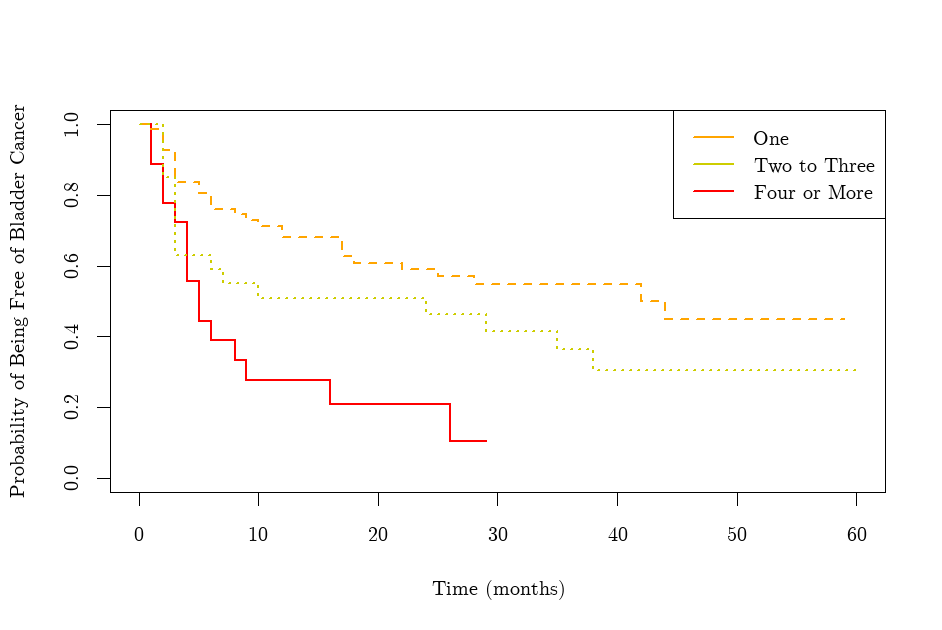
\includegraphics[width=\linewidth]{graphs/case1/recurrance~tumor_count.png}
		  \caption{\textbf{Figure 6.} Time to Recurrence by Number of Initial Tumors}
		  \label{surv-tumor-count}
		\end{subfigure}
		\hfill
		\begin{subfigure}[t]{0.48\textwidth}
		  \centering
		  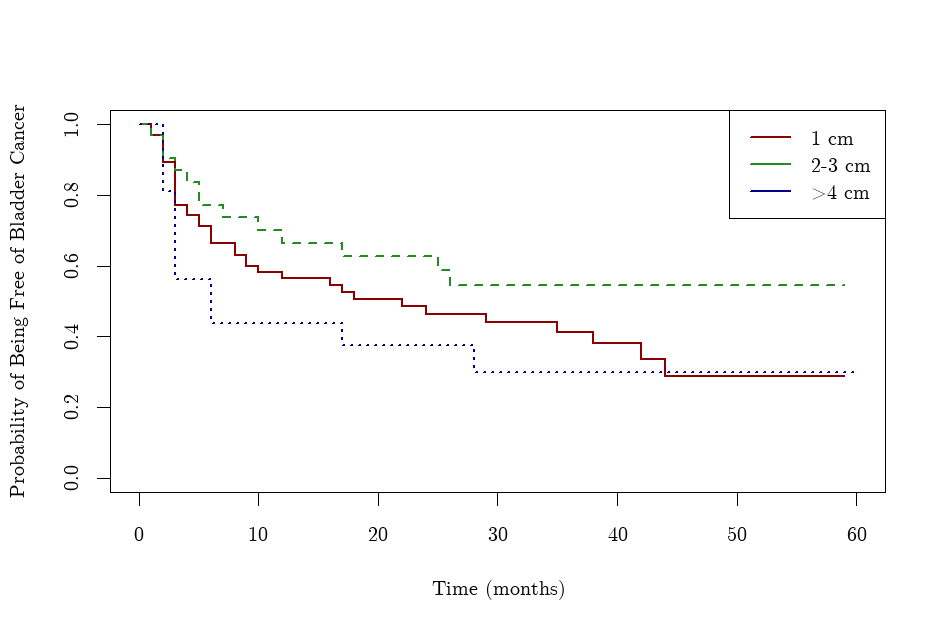
\includegraphics[width=\linewidth]{graphs/case1/recurrance~tumor_size.png}
		  \caption{\textbf{Figure 7.} Time to Recurrence by Size of Initial Tumors}
		  \label{surv-tumor-size}
		\end{subfigure}
		\caption{Figures 6-7: Kaplan-Meier Estimates of Time to Bladder Cancer Recurrence by Number \& Size of Initial Tumors}
	\end{figure}
	\addtocounter{figure}{1}

	\subsection*{Discussion}
	Neither pyridoxine or thiotepa made a significant impact in changing the time to recurrence of cancer or survival times in subjects. While there may be other clinical benefits associated with these two treatments of bladder cancer, alternative treatments should be considered in the search for methods to prevent the recurrence of bladder cancer. Other studies also suggested that pyridoxine and thiotepa were ineffective treatments in this situation (Newling et. al., 2017). 

	One limitation of our study was the low number of study participants. Additionally, while we stopped following subjects after we observed recurrence of cancer, it may be worth continuing to follow them to see if they die. This helps avoid any potential biases related to non-informative censoring, especially in analysis of how impactful the two treatments are on survival rates of patients specifically.

	There exist a large number of potential confounders outside of the scope of the study that are worth exploring. We found interaction between the number of tumors previously present in a subject and the time to cancer recurrence. Thus, the number of tumors present an important confounding variable that should be explored further through adjustment or stratification in future research. On the contrary, the size of tumors in subjects did not appear to impact time to cancer recurrence. Patient characteristics— demographic attributes, physical activity, and smoking status— are all potential confounding variables that are known risk factors for cancer (Rink et. al., 2013). A more important factor that was not considered in this study was the stage of cancer in patients, which could have a drastic impact on cancer remission and recurrence.

	\newpage
	\subsection*{Appendix}
	\begin{itemize}
		\item Newling, D. W. W., Robinson, M. R. G., Smith, P. H., Byar, D., Lockwood, R., Stevens, I., De Pauw, M., \& Sylvester, R. (2017). Tryptophan metabolites, pyridoxine (vitamin B(6)) and their influence on the recurrence rate of superficial bladder cancer. \textit{European Urology}, 27(2), 110–116. \url{https://doi.org/10.1159/000475139}
		
		\item Rink, M., Zabor, E. C., Furberg, H., Xylinas, E., Ehdaie, B., Novara, G., \ldots \& Shariat, S. F. (2013). Impact of smoking and smoking cessation on outcomes in bladder cancer patients treated with radical cystectomy. \textit{European Urology}, 64(3), 456-464.
	\end{itemize}

	\subsection*{R Code}

	\begin{lstlisting}[language=R,caption={Case 1: Bladder Cancer Survival Analysis},label={lst:case1}]
		## case 1 ##
library(survival)
# libraries and code for fancy graph formatting
library(showtext)
library(DescTools)
library(Rfit)
font_add(family = 'ComputerModern', regular = 'cmunrm.ttf') #for consistent formatting in LaTex
showtext_auto()
par(family = 'ComputerModern')
# end formatting stuff
## case 1 ##

blad <- read.csv('bladder.txt', header=TRUE, sep='')

## Part 1. first recurrence of cancer by treatment group

recur  <- survfit(Surv(time, status1) ~ treatment, data = blad)
recur

# Figure 1. Kaplan-Meier Estimate of Time to Recurrence in Subjects by Treatment
plot(recur, col = c('purple', 'green3', 'blue'), lty = c(1,2,3), 
     main = '', xlab = 'Time (months)',
     ylab = 'Probability of Being Free of Bladder Cancer', lwd = 2)
legend('topright', legend = c('Placebo', 'Pyridoxine', 'Thiotepa'), 
       col = c('purple', 'green3', 'blue'), lty = c(1,2,3), lwd = 2)

# wilcoxon test for treatment
survdiff(Surv(time, status1) ~ treatment, data = blad, rho = 1) 

########## More Graphs ====================================
par(cex = 1.5)

placebo = subset(blad, treatment == 'placebo')
surv_plac = survfit(Surv(time, status1) ~ 1, data = placebo)

plot(surv_plac, 
     col = 'purple', lty = 1, lwd = 2, main = '', xlab = 'Time (months)', 
     ylab = 'Probability of Being\nFree of Bladder Cancer')
legend('topright', legend = c('Placebo', '95% CI'),
       col = 'purple', lty = c(1,2), lwd = 2)

#pyridoxine
pyrid = subset(blad, treatment == 'pyridoxine')
surv_pyrid = survfit(Surv(time, status1) ~ 1, data = pyrid)

plot(surv_pyrid, 
     col = 'green3', lty = 1, lwd = 2, main = '', xlab = 'Time (months)', 
     ylab = 'Probability of Being\nFree of Bladder Cancer')
legend('topright', legend = c('Pyridoxine', '95% CI'),
       col = 'green3', lty = c(1,2), lwd = 2)

#thiotepa
#genuinely have no idea how the spellings for these drugs were made
thi = subset(blad, treatment == 'thiotepa')
surv_thi = survfit(Surv(time, status1) ~ 1, data = thi)

plot(surv_thi, 
     col = 'blue', lty = 1, lwd = 2, main = '', xlab = 'Time (months)', 
     ylab = 'Probability of Being\nFree of Bladder Cancer')
legend('topright', legend = c('Thiotepa', '95% CI'),
       col = 'blue', lty = c(1,2), lwd = 2)

######## end of individual graphs section


# chi square association test to see if censoring rates differed
table(blad$treatment, blad$status1)
chisq.test(table(blad$treatment, blad$status1))
# censoring rates did not occur

########## cumulative hazard functions (might not include)
plot(recur, col = c('darkorchid4', 'darkgreen', 'darkblue'), lty = c(1,2,3), 
     main = 'Cumulative Hazard First Recurrence by Treatment', xlab = 't', lwd = 2,
     fun = 'cumhaz')
title(ylab = expression(hat(H)(t)), line = 2.5)
legend('bottomright', legend = c('Placebo', 'Pyridoxine', 'Thiotepa'), 
       col = c('darkorchid4', 'darkgreen', 'darkblue'), lty = c(1,2,3), lwd = 2)



## survival analysis of death by treatment group
death  <- survfit(Surv(time, status2) ~ treatment, data = blad)
death

plot(death, col = c('darkorchid4', 'darkgreen', 'navy'), lty = c(1,2,3), 
     main = '', xlab = 'Time (months)', lwd = 2,
     ylab = 'Probability of Survival')
legend('bottomleft', legend = c('Placebo', 'Pyridoxine', 'Thiotepa'), 
       col = c('darkorchid4', 'darkgreen', 'navy'), lty = c(1,2,3), lwd = 2)

survdiff(Surv(time, status2) ~ treatment, data = blad, rho = 1) 
table(blad$treatment, blad$status2)
chisq.test(table(blad$treatment, blad$status2))


######################## cumulative hazard ##########################
## https://r-charts.com/colors/

plot(death, col = c('purple3', 'forestgreen', 'blue3'), lty = c(1,2), 
     main = 'Cumulative Hazard of Death by Treatment', xlab = 'Time (months)', lwd = 2,
     fun = 'cumhaz')
title(ylab = expression(hat(H)(t)), line = 2.5)
legend('topleft', legend = c('Placebo', 'Pyridoxine', 'Thiotepa'), 
       col = c('purple3', 'forestgreen', 'blue3'), lty = c(1,2,3), lwd = 2)


################## interactors/confounders
############### first recurrence by number of tumors
number_recur  <- survfit(Surv(time, status1) ~ number, data = blad)
number_recur


sum(blad$number == 'Two to Three' )

plot(number_recur, col = c('red', 'orange', 'yellow3'), lty = c(1,2,3), 
     main = 'Recurrence by Tumor Number', xlab = 'Time (months)', lwd = 2)
title(ylab = expression(hat(S)(t)), line = 2.5)
legend('topright', legend = c('1 Tumor', '2 or 3 Tumors', '4+ Tumors'), 
       col = c('red', 'orange', 'yellow3'), lty = c(1,2,3), lwd = 2)

survdiff(Surv(time, status1) ~ number, data = blad, rho = 1)
table(blad$number, blad$status1)
chisq.test(table(blad$number, blad$status1))



### first recurrence by size of tumors 
size_recur  <- survfit(Surv(time, status1) ~ size, data = blad)
size_recur 


plot(size_recur, col = c('red', 'forestgreen', 'blue'), lty = c(1,2,3), 
     main = 'Bladder Survival for Size', xlab = 'Time (months)', lwd = 2)
title(ylab = expression(hat(S)(t)), line = 2.5)
legend('topright', legend = c('1cm', '2cm to 3cm', '4cm or Larger'), 
       col = c('red', 'forestgreen', 'blue'), lty = c(1,2,3), lwd = 2)


survdiff(Surv(time, status1) ~ size, data = blad, rho = 1)
table(blad$size, blad$status1)
chisq.test(table(blad$size, blad$status1))




	\end{lstlisting}

	\newpage
	\setcounter{table}{0}
	\setcounter{figure}{0}

	\subsection*{Background}
	Chronic granulomatous disease or CGD is a genetic disorder in which white blood cells called phagocytes are unable to kill certain types of bacteria and fungi. Consequently, patients suffering from CGD are subject to frequent and potentially life-threatening infections. CGD impacts the effectiveness of phagocytes, a type of white blood cell, that makes patients more susceptible to bacterial and fungal infections. We conducted a placebo controlled trial of a cytokine-based treatment using interferon gamma to examine its effect on recurrence of CGD. The primary endpoint of the study was the first recurrence of a bacterial or fungal infection and the secondary endpoint was the second recurrence of infection. The pattern of inheritance and use of antibiotics may impact recurrence as well. In total, 128 patients were available for analysis of the primary endpoint while only 44 patients were available for the secondary endpoint.

	\subsection*{Methods}
	128 patients suffering from CGD were selected for this randomized controlled trial to determine the effectiveness of interferon-gamma on disease outcomes. To examine the risk over time of developing a bacterial or fungal infection in the two study arms, we used Kaplan-Meier estimation to estimate time to infection. We used the Gehan-Breslow-Wilcoxon test to analyze whether there was a difference between the survival curves.

	In addition to time to a first infection, we also analyzed the time to a second infection in patients where we observed a first infection. A person’s use of prophylactic antibiotics during the study may have impacted their resulting time to infection. Additionally, chronic granulomatous disease is a unique genetic disease in that it has two patterns of inheritance. CGD can either be X-linked or autosomal, with X-linked versions of the disease being far more severe. To examine the potential interaction and confounding effect of these two factors, we estimated time to infection functions using Kaplan-Meier estimation as additional secondary analyses for this study. All testing was done at the nominal level.

	\subsection*{Results}
	Among the 128 patients who were available for the primary endpoint, 63 received the Cytokine-based treatment the remaining 65 formed the placebo control group. 44 of the subjects had a first recurrence of infection under study observation, and 84 were censored. We only observed the median time to first infection recurrence in patients receiving the placebo of 204 days. Of the total 128 patients, only 34 experienced a second recurrence of infection, with 14 of those receiving the treatment and 30 receiving the placebo. We did not observe a median survival time for patients receiving the Cytokine-based treatment with the first recurrence or for both groups with the second occurance of infection, as the observed infection counts in this group treatment arm were very low. 

	\begin{table}[ht]
		\centering
		\footnotesize
		\caption{Time to First Infection of Patients by Treatment Group}
		\begin{tabular}{lccc}
		\toprule
		\textbf{Treatment} & \textbf{Number of Patients} & \textbf{Observed Infections} & \textbf{Median Time to Infection} \\
		\midrule
		Cytokine-based Treatment & 63 & 14 & NA \\
		Placebo & 65 & 30 & 304 \\
		\midrule
		Total & 128 & 44 & \\
		\bottomrule
		\end{tabular}
	\end{table}

	
	\begin{figure}[h]
		\centering
		\tiny
		  \centering
		  \tiny
		  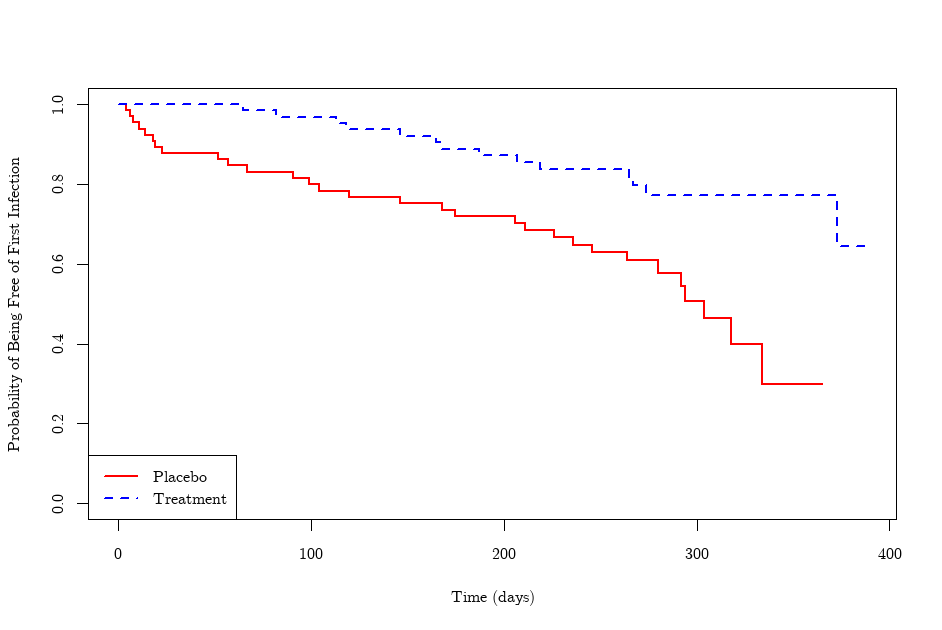
\includegraphics[width=0.4\textwidth]{graphs/case2/infection~treatment.png}
		  \caption{Kaplan-Meier Estimates of Time to First Infection by Treatment}
		  \label{fig1}
	\end{figure}

	\newpage

	\begin{figure}[htbp]
		\centering
		\captionsetup{labelformat = empty}
		\begin{subfigure}[t]{0.48\textwidth}
			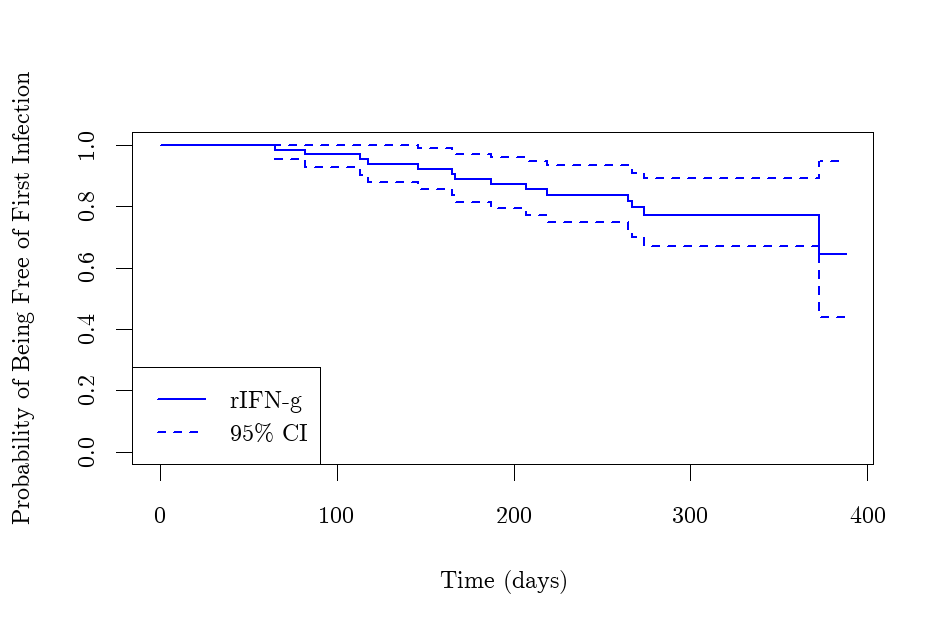
\includegraphics[width=\linewidth]{graphs/case2/infection~treatment_rIFN.png}
			\caption*{\raggedright\hyphenpenalty=10000\exhyphenpenalty=10000\sloppy 
			\textbf{Figure 2.} Time to Infection in Subjects Treated with Interferon-Gamma Therapy}
		\end{subfigure}
		\hfill
		\begin{subfigure}[t]{0.48\textwidth}
			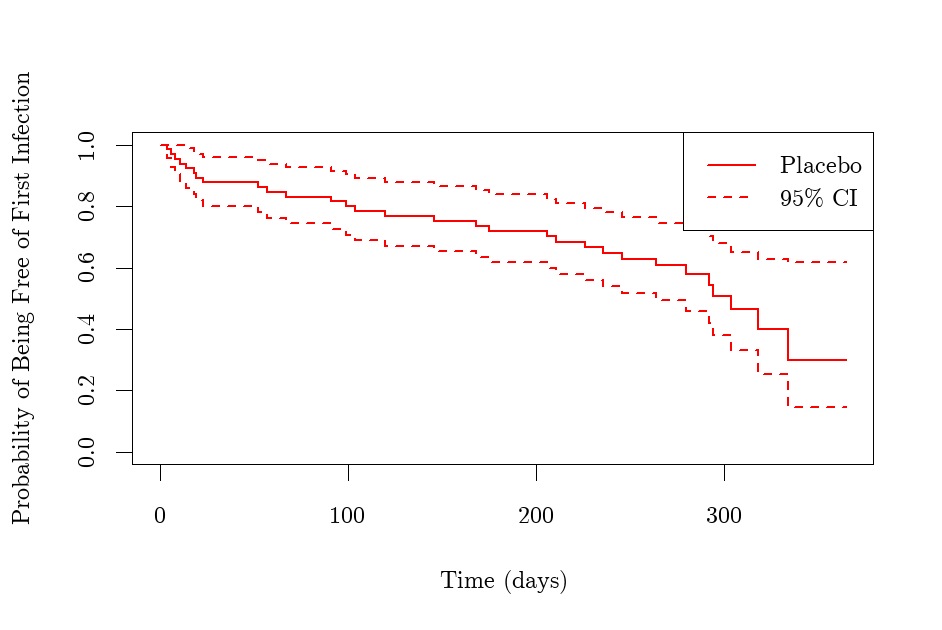
\includegraphics[width=\linewidth]{graphs/case2/infection~treatment_placebo.png}
			\caption*{\raggedright\hyphenpenalty=10000\exhyphenpenalty=10000\sloppy 
			\textbf{Figure 3.} Time to Infection in Subjects in Control Group}
		\end{subfigure}
		\caption{Figures 2-3: Kaplan-Meier Estimates of Time to Infection for Treatment \& Placebo Groups}
		\label{fig:recurrence_treatment_groups}
	\end{figure}
	\addtocounter{figure}{1}

	We found a statistically significant difference in first recurrence rates over time between the two treatment groups $(p $<$0.001, \chi^2 = 11.3$, df = 1). Figure 1 shows the Kaplan-Meier estimates of time to a first infection. Additionally, we did not find a significant difference in second recurrence rates between the two treatment groups $(p = 0.7, \chi^2 = 0.1$, df = 1). Figure 4 shows the estimate of second recurrence rates over the study.

	\begin{table}[ht]
		\centering
		\footnotesize
		\caption{Time to Second Infection of Patients by Treatment Group}
		\begin{tabular}{lccc}
		\toprule
		\textbf{Treatment} & \textbf{Number of Patients} & \textbf{Observed Infections} & \textbf{Median Time to Infection} \\
		\midrule
		Cytokine-based Treatment & 14 & 5 & NA \\
		Placebo & 30 & 12 & NA \\
		\midrule
		Total & 44 & 17 & \\
		\bottomrule
		\end{tabular}
	\end{table}

	\begin{figure}[H]
		\centering
		\tiny
		  \centering
		  \tiny
		  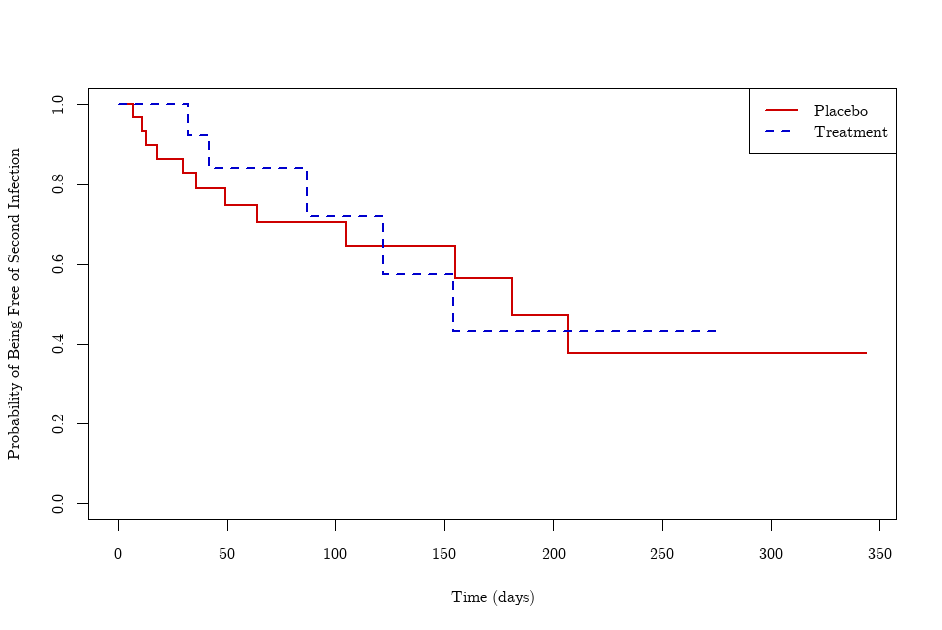
\includegraphics[width=0.6\textwidth]{graphs/case2/2nd_infection.png}
		  \caption{Kaplan-Meier Estimates of Time to Second Infection by Treatment}
		  \label{fig1}
	\end{figure}

	\begin{table}[H]
		\centering
		\footnotesize
		\caption{Time to First Infection of Patients by Genetic Inheritance Pattern}
		\begin{tabular}{lccc}
		\toprule
		\textbf{Pattern of Inheritance} & \textbf{Number of Patients} & \textbf{Observed Infections} & \textbf{Median Time to Infection} \\
		\midrule
		Autosomal & 42 & 16 & NA \\
		X-Linked & 86 & 28 & 373 \\
		\midrule
		Total & 128 & 44 & \\
		\bottomrule
		\end{tabular}
	\end{table}

	While 42 of the 128 subjects only had an Autosomal pattern of inheritance, 86 had an X-linked pattern. Only the X-linked group had a measure of median time to the primary endpoint of analysis at 373 days. There was not a statistically significant difference in time to the first recurrence of infection based on the patient’s pattern of inheritance $(p =0.6, \chi^2 = 0.2$, df = 1). Figure 5 shows the Kaplan-Meier estimates of the time to infection by inheritance pattern.

	\begin{figure}[htbp]
		\centering
		\captionsetup{labelformat = empty}
		\begin{subfigure}[t]{0.48\textwidth}
			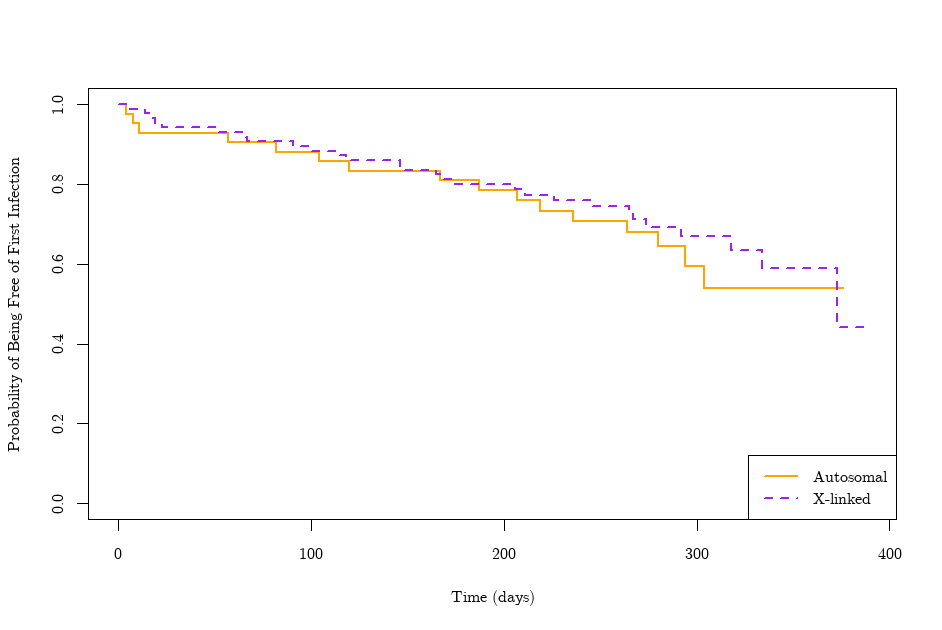
\includegraphics[width=\linewidth]{graphs/case2/infection~inheritance.png}
			\caption*{\raggedright\hyphenpenalty=10000\exhyphenpenalty=10000\sloppy 
			\textbf{Figure 5.} Time to Infection by CGD Inheritance}
		\end{subfigure}
		\hfill
		\begin{subfigure}[t]{0.48\textwidth}
			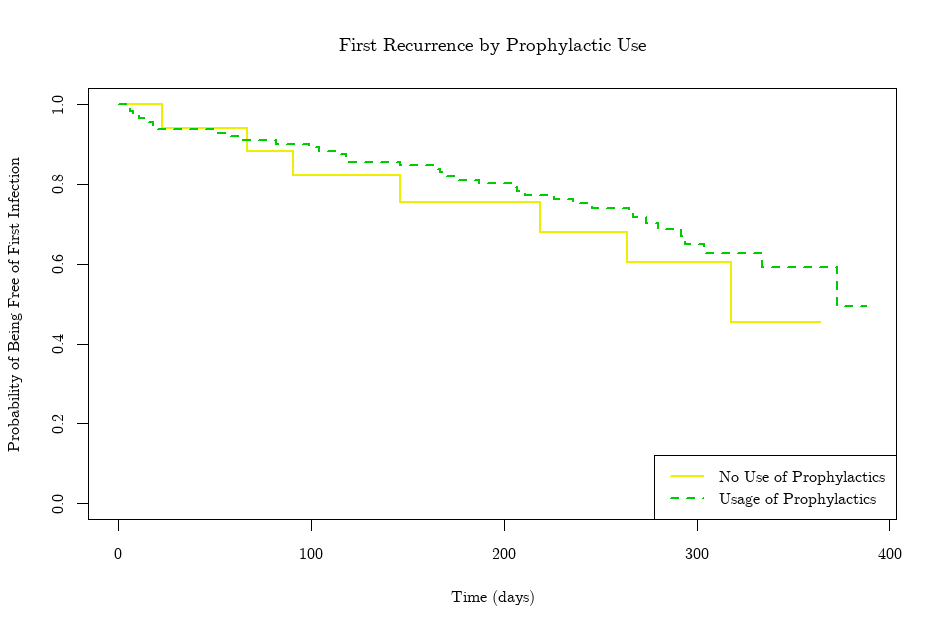
\includegraphics[width=\linewidth]{graphs/case2/infection~prop_use.png}
			\caption*{\raggedright\hyphenpenalty=10000\exhyphenpenalty=10000\sloppy 
			\textbf{Figure 6.} Time to Infection by Prophylactic Usage}
		\end{subfigure}
		\caption{Figures 2-3: Kaplan-Meier Estimates of Time to Infection by CGD Inheritance Status \& Prophylactic Usage}
		\label{fig:recurrence_treatment_groups}
	\end{figure}
	\addtocounter{figure}{1}


	\begin{table}[ht]
		\centering
		\footnotesize
		\caption{Time to First Infection of Patients by Prophylactic Antibiotic Usage at Study Entry}
		\begin{tabular}{lccc}
		\toprule
		\textbf{Use of Prophylactic Antibiotics} & \textbf{Number of Patients} & \textbf{Observed Infections} & \textbf{Median Time to Infection} \\
		\midrule
		Yes Usage & 111 & 37 & 373 \\
		No Usage & 17 & 7 & 318 \\
		\midrule
		Total & 128 & 44 & \\
		\bottomrule
		\end{tabular}
	\end{table}
	
	111 of the 128 patients were using prophylactic antibiotics at study entry, while the remaining 17 were not. Of those using, 37 had an observed first recurrence of infection, and 7 of the 17 not using antibiotics had a first recurrence. The median time to first infection for the usage and non-usage groups were 373 and 318 days, respectively. Figure 6 shows the Kaplan-Meier survival curve of time to first infection in patients, separated by their prophylactic usage. We did not find evidence to suggest that the usage of prophylactic antibiotics at study entry had an impact on the time to first recurrence of infection $(p = 0.4, \chi^2 = 0.7$, df = 1).

	\subsection*{Discussion}
	Of our statistical analysis of treatment groups and potential confounding variables, only the treatment group and time to the first recurrence of infection were significantly related. Subjects in the interferon gamma treatment group had a significantly longer time to first occurrence. This suggests that interferon-gamma therapy works as a treatment for chronic granulomatous disease. However, we found that therapy had no significant impact on the time to a second infection. Other clinical research also suggests that interferon-gamma treatment has a protective impact on people suffering with CGD (Errante et al., 2008). However, we found that therapy had no significant impact on the time to a second infection. 

	Our study was limited by the sample size and non-informative censoring, which was a potential bias especially when it came to observing second infections. Patients in the cytokine-based treatment group had a higher than expected censoring rate when measuring the time to first recurrence, which suggest adverse side effects of the treatment. Further studies should be done to understand these side effects in more detail. While we did not find that genetic inheritance patterns or prophylactic usage were confounders in this study, other confounding factors such as other biological characteristics or personal behavior should be considered in further research.

	\newpage
	\subsection*{Appendix}

	\begin{itemize}
		\item Errante, P. R., Frazao, J. B., \& Antonio Condino-Neto. (2008). The Use of Interferon-Gamma Therapy in Chronic Granulomatous Disease. \textit{Recent Patents on Anti-Infective Drug Discovery}, 3(3), 225--230. \url{https://doi.org/10.2174/157489108786242378}
	\end{itemize}

	\subsection*{R Code}
	\begin{lstlisting}[language=R, basicstyle=\ttfamily\footnotesize, breaklines=true]
		## case 2 ##
		library(survival)
		# libraries and code for fancy graph formatting
		library(showtext)
		library(DescTools)
		library(Rfit)
		font_add(family = 'ComputerModern', regular = 'cmunrm.ttf') #for consistent formatting in LaTex
		showtext_auto()
		par(family = 'ComputerModern')
		# end formatting stuff
		
		firstr <- read.csv('cgd1.txt', header=TRUE, sep='')
		secondr <- read.csv('cgd2.txt', header=TRUE, sep='')
		
		## First infection by treatment group 
		first_treat  <- survfit(Surv(time, status) ~ treatment, data = firstr)
		first_treat 
		first_treat$strata
		
		plot(first_treat, col = c('red', 'blue'), lty = c(1,2,3), 
			 main = '', xlab = 'Time (days)', 
			 ylab = 'Probability of Being Free of First Infection', lwd = 2)
		legend('bottomleft', legend = c('Placebo', 'Treatment'), 
			   col = c('red', 'blue'), lty = c(1,2,3), lwd = 2)
		
		survdiff(Surv(time, status) ~ treatment, data = firstr, rho = 1)
		
		table(firstr$treatment, firstr$status)
		chisq.test(table(firstr$treatment, firstr$status))
		
		#### cumulative hazard
		plot(first_treat, col = c('red', 'blue'), lty = c(1,2,3), 
			 main = 'Cumulative Hazard \nof First Infection by Treatment', xlab = 'Time (days)',
			 ylab = 'Probability of Being\nFree of First Infection', lwd = 2,
			 fun = 'cumhaz')
		legend('topleft', legend = c('Placebo', 'Treatment'), 
			   col = c('red', 'blue'), lty = c(1,2,3), lwd = 2)
		
		#####
		par(cex = 1.5)
		
		placebo = subset(firstr, treatment == 'placebo')
		surv_plac = survfit(Surv(time, status) ~ 1, data = placebo)
		
		plot(surv_plac, 
			 col = 'red', lty = 1, lwd = 2, main = '', xlab = 'Time (days)', 
			 ylab = 'Probability of Being Free of First Infection')
		legend('topright', legend = c('Placebo', '95% CI'),
			   col = 'red', lty = c(1,2), lwd = 2)
		
		# treatment
		pyrid = subset(firstr, treatment == 'rIFN-g')
		surv_rIFNg = survfit(Surv(time, status) ~ 1, data = pyrid)
		
		plot(surv_rIFNg, 
			 col = 'blue', lty = 1, lwd = 2, main = '', xlab = 'Time (days)', 
			 ylab = 'Probability of Being Free of First Infection')
		legend('bottomleft', legend = c('rIFN-g', '95% CI'),
			   col = 'blue', lty = c(1,2), lwd = 2)
		
		######## end of individual graphs section
		
		## Second infection by treatment group 
		par(cex = 1)
		second_treat  <- survfit(Surv(time, status) ~ treatment, data = secondr)
		second_treat 
		second_treat$strata
		
		plot(second_treat, col = c('red3', 'blue3'), lty = c(1,2,3), 
			 main = '', xlab = 'Time (days)',
			 ylab = 'Probability of Being Free of Second Infection', lwd = 2)
		legend('topright', legend = c('Placebo', 'Treatment'), 
			   col = c('red3', 'blue3'), lty = c(1,2,3), lwd = 2)
		
		survdiff(Surv(time, status) ~ treatment, data = secondr, rho = 1)
		table(secondr$treatment, secondr$status)
		chisq.test(table(secondr$treatment, secondr$status))
		
		## cumulative hazard function
		plot(second_treat, col = c('red3', 'blue3'), lty = c(1,2,3), 
			 main = 'Cumulative Hazard \nof Second Infection by Treatment', xlab = 'Time (days)',
			 ylab = 'Probability of Being\nFree of Second Infection', lwd = 2,
			 fun = 'cumhaz')
		legend('bottomright', legend = c('Placebo', 'Treatment'), 
			   col = c('red3', 'blue3'), lty = c(1,2,3), lwd = 2)
		
		## First recurrence by inherit group 
		first_inherit  <- survfit(Surv(time, status) ~ inherit, data = firstr)
		first_inherit 
		first_inherit$strata
		
		#### confounders: genetics and prop. use
		plot(first_inherit, col = c('orange', 'purple'), lty = c(1,2), 
			 main = '', xlab = 'Time (days)',
			 ylab = 'Probability of Being Free of First Infection', lwd = 2)
		legend('bottomright', legend = c('Autosomal', 'X-linked'), 
			   col = c('orange', 'purple'), lty = c(1,2,3), lwd = 2)
		
		survdiff(Surv(time, status) ~ inherit, data = firstr, rho = 1)
		table(firstr$inherit, firstr$status)
		chisq.test(table(firstr$inherit, firstr$status))
		
		## First recurrence by prophylactic use group 
		first_prop  <- survfit(Surv(time, status) ~ propylac, data = firstr)
		first_prop
		first_prop$strata
		
		plot(first_prop, col = c('yellow2', 'green3'), lty = c(1,2,3), 
			 main = 'First Recurrence by Prophylactic Use', xlab = 'Time (days)',
			 ylab = 'Probability of Being Free of First Infection', lwd = 2)
		legend('bottomright', legend = c('No Use of Prophylactics', 'Usage of Prophylactics'), 
			   col = c('yellow2', 'green3'), lty = c(1,2,3), lwd = 2)
		
		survdiff(Surv(time, status) ~ propylac, data = firstr, rho = 1)
		table(firstr$propylac, firstr$status)
		chisq.test(table(firstr$propylac, firstr$status))
		\end{lstlisting}
		




		
\end{document}














